\documentclass[conference]{IEEEtran}
\IEEEoverridecommandlockouts
\usepackage{cite}
\usepackage{amsmath,amssymb,amsfonts}
\usepackage{algorithmic}
\usepackage{graphicx}
\usepackage{textcomp}
\usepackage{listings}
\usepackage{xcolor}

\newcommand{\csh}{C{\#}}

\def\BibTeX{{\rm B\kern-.05em{\sc i\kern-.025em b}\kern-.08em
    T\kern-.1667em\lower.7ex\hbox{E}\kern-.125emX}}

\begin{document}

\title{Creating 3D games with Unity3D}

\author{\IEEEauthorblockN{1\textsuperscript{st} Boris Fuchs}
\IEEEauthorblockA{\textit{Mobile Computing} \\
\textit{University of Applied Sciences Upper Austria}\\
Hagenberg, Austria \\
boris.fuchs@students.fh-hagenberg.at}
\and
\IEEEauthorblockN{2\textsuperscript{nd} David Mitterlehner}
\IEEEauthorblockA{\textit{Mobile Computing} \\
\textit{University of Applied Sciences Upper Austria}\\
Hagenberg, Austria \\
david.mitterlehner@students.fh-hagenberg.at}
\and
\IEEEauthorblockN{3\textsuperscript{rd} Anika Seibezeder}
\IEEEauthorblockA{\textit{Mobile Computing} \\
\textit{University of Applied Sciences Upper Austria}\\
Hagenberg, Austria \\
anika.seibezeder@students.fh-hagenberg.at}
}

\maketitle

\begin{abstract}
\emph{Lorem ipsum dolor sit amet, consetetur sadipscing elitr, sed diam nonumy eirmod tempor invidunt ut labore et dolore magna aliquyam erat, sed diam voluptua. At vero eos et accusam et justo duo dolores et ea rebum. Stet clita kasd gubergren, no sea takimata sanctus est Lorem ipsum dolor sit amet. Lorem ipsum dolor sit amet, consetetur sadipscing elitr, sed diam nonumy eirmod tempor invidunt ut labore et dolore magna aliquyam erat, sed diam voluptua. At vero eos et accusam et justo duo dolores et ea rebum. Stet clita kasd gubergren, no sea takimata sanctus est Lorem ipsum dolor sit amet.}
\end{abstract}

\begin{IEEEkeywords}
component, formatting, style, styling, insert
\end{IEEEkeywords}

\section{Introduction}
Nowadays creating realistic 3D games is getting a lot easier, due to various tools like Unity3D or the Unreal Engine. Game developers need little to no programming skills to make games in a minimum amount of time, because a great amount of premade assets and scripts are available for a very low cost. Most of the developing work can be done in the graphical editor, like creating 3D figures and adding properties, which can include self made scripts or physical properties. The majority of the existing game editors provide developing on multiple platforms including Smartphones and the most common game consoles. However Unity3D is better suited for devices with low end graphics cards, because it is more lightweight than the Unreal Engine. Compared to it, the available assets of Unity3D are not as high quality, but more economical on memory and graphics. \\ \\
The main points of this paper are: outlining the workflow of the game development process in Unity3D which consists of creating an environment, making a Third-Person-Character and some enemies, and comparing the basic functionality and simplicity of Unity3D and the Unreal Engine. The advantages and disadvantages of both editors are examined and demonstrated. \\
The first point of the game development process in Unity3D is to create an environment, with a small forest, some mountains and a few cottages. Then some textures are added to the components.
Secondly the Third-Person-Character is linked with a  script, so it can move around in the environment.
The third point is to create some enemies, that are chasing the player. 
Lastly animations for both, the character and the enemies, are provided and added to the game. \\ \\
The goal of this paper is to demonstrate the simplicity of Unity3D by creating a small 3D game in Unity3D.To keep the costs low, only freely available assets are used. The focus is not on scripting, but on the features of the graphical editor provided by Unity3D and the Unreal Engine. 


\section{Creating an Environment}

\subsection{Subsection 1}

\emph{Lorem ipsum dolor sit amet, consetetur sadipscing elitr, sed diam nonumy eirmod tempor invidunt ut labore et dolore magna aliquyam erat, sed diam voluptua. At vero eos et accusam et justo duo dolores et ea rebum. Stet clita kasd gubergren, no sea takimata sanctus est Lorem ipsum dolor sit amet. Lorem ipsum dolor sit amet, consetetur sadipscing elitr, sed diam nonumy eirmod tempor invidunt ut labore et dolore magna aliquyam erat, sed diam voluptua. At vero eos et accusam et justo duo dolores et ea rebum. Stet clita kasd gubergren, no sea takimata sanctus est Lorem ipsum dolor sit amet.
Lorem ipsum dolor sit amet, consetetur sadipscing elitr, sed diam nonumy eirmod tempor invidunt ut labore et dolore magna aliquyam erat, sed diam voluptua. At vero eos et accusam et justo duo dolores et ea rebum. Stet clita kasd gubergren, no sea takimata sanctus est Lorem ipsum dolor sit amet. Lorem ipsum dolor sit amet, consetetur sadipscing elitr, sed diam nonumy eirmod tempor invidunt ut labore et dolore magna aliquyam erat, sed diam voluptua. At vero eos et accusam et justo duo dolores et ea rebum. Stet clita kasd gubergren, no sea takimata sanctus est Lorem ipsum dolor sit amet.
Lorem ipsum dolor sit amet, consetetur sadipscing elitr, sed diam nonumy eirmod tempor invidunt ut labore et dolore magna aliquyam erat, sed diam voluptua. At vero eos et accusam et justo duo dolores et ea rebum. Stet clita kasd gubergren, no sea takimata sanctus est Lorem ipsum dolor sit amet. Lorem ipsum dolor sit amet, consetetur sadipscing.}

\section{Character Controls}

Character controls are a must have when developing a game. Otherwise the user would not be able to interact with a given character. No matter how hard the user is pressing a key or moving the mouse, the character still would not move at all.
With Unity3D the user interaction can be easily made by implementing scripts and adding them to the editor via Drag and Drop. The scripts can be written in \csh, JavaScript and Boo \cite{b1}. In the editor itself there is no opportunity to write the code, but there are several supported editors such as the recommended editor MonoDevelop by Unity3D or VisualStudio by Microsoft \cite{b1}.

\subsection{Adding a Character}

In Unity3D adding a character is easily done by dragging a Prefab or an object into the middle screen to the wanted position. There is also another possibility by dragging the Prefab or object to the left side of the screen, where all used objects are shown. A Prefab is a pre-built object combined of one to many components \cite{b2}. When downloading the Unity3D editor some prefabs are already given and can be used as is.
To see and edit features of the Prefab or object, a left click on the wanted object on the left side of the screen is needed. 

\begin{figure}[htbp]
  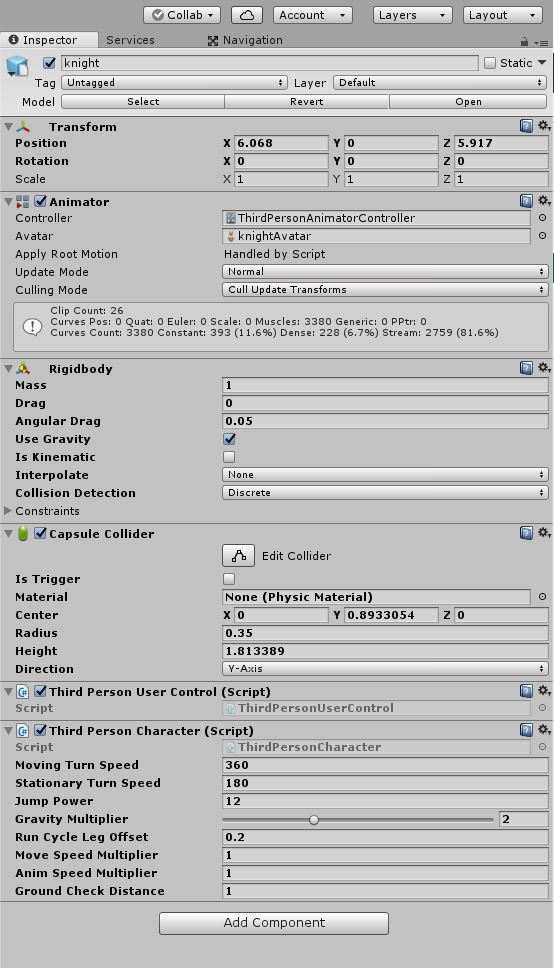
\includegraphics[width=.4\textwidth]{pictures/character_controls_character_components}
  \caption{Character Components}
  \label{fig:character_controls_character_components}
\end{figure}

As seen in figure~\ref{fig:character_controls_character_components}, a character has components like a Rigidbody, which gives the character a mass, a capsule collider, which triggers interrupts when colliding with other objects and scripts. Scripts can have some changeable variables like shown with the 2\textsuperscript{nd} script, or no changeable variable.

\lstloadlanguages{[Sharp]C}
\lstset{
basicstyle=\ttfamily\small,
numbers=left,
breaklines=true,
numberstyle=\tiny,
numbersep=5pt,
tabsize=3
}
\definecolor{listinggray}{gray}{0.95}
\definecolor{keyword}{rgb}{0.4, 0, 0.1}
\definecolor{comment}{rgb}{0, 0.4, 0}

\lstset{keywordstyle=\color{keyword}\bfseries}
\lstset{commentstyle=\color{comment}}
\lstset{backgroundcolor=\color{listinggray}}
\lstset{language=[Sharp]C}

\subsection{Scripting in VisualStudio}

A script is simply added by clicking the button "Add Component", choosing "New Script" and selecting the wanted language. After adding the script it can be written by double clicking the component and opening the wanted script editor. \\
The first thing to know about writing a script for Unity3D is, that the class is extending from the \lstinline!class MonoBehaviour! and is ipmlementing the functions \lstinline!void Start()!, \lstinline!void Update()! and \lstinline!void FixedUpdate()!. 
The start function is used for variable initialization and one time execution.
The update function is used for continuous events, like checking which key is pressed, and is updated every frame\cite{b1}. As the user may press other keys while playing the game, the statements for checking the key should be implemented in the update function. Both functions are not necessarily needed but can help building the logic of the game.
Another important function is \lstinline!void FixedUpdate()!. Like the \lstinline!void Update()! function, it also is updated every frame and it is mainly used when dealing with the Physics of the Object \cite{b1}. \\
When adding variables there is just a few thing to know: all \lstinline!public! variables are later shown in the component screen and can be edited there. It is also possible to import other components from the object. They are added to by using \lstinline!GetComponent<>()!

\subsection{Cross Platform Input Manager}

The Cross Platform Input Manager can be used to determine how keys or actions should be interpreted. For example there can be an entry considering jumping with a character, which defines, that a jump on a Desktop or Laptop is made with pressing the spacebar, while on the smartphone a touch gesture activates the jump. After defining the inputs, they can be used with \lstinline!CrossPlatformInputManager.GetButtonDown("Jump")!. \\

\begin{lstlisting}[caption=Example Implementation for Determining a Jump,label=list:character_controls_jump_implementation]
private bool isJumping;

private void Update()
{
	if (!isJumping)
	{
		isJumping = CrossPlatformInputManager.GetButtonDown("Jump");
	}
}
\end{lstlisting}

The code in Listing~\ref{list:character_controls_jump_implementation} shows how to implement the Cross Platform Input Manager in the \lstinline!void Update()! function which is updated every frame. 

\section{Adding Animations}

\emph{Lorem ipsum dolor sit amet, consetetur sadipscing elitr, sed diam nonumy eirmod tempor invidunt ut labore et dolore magna aliquyam erat, sed diam voluptua. At vero eos et accusam et justo duo dolores et ea rebum. Stet clita kasd gubergren, no sea takimata sanctus est Lorem ipsum dolor sit amet. Lorem ipsum dolor sit amet, consetetur sadipscing elitr, sed diam nonumy eirmod tempor invidunt ut labore et dolore magna aliquyam erat, sed diam voluptua. At vero eos et accusam et justo duo dolores et ea rebum. Stet clita kasd gubergren, no sea takimata sanctus est Lorem ipsum dolor sit amet.}

\section{Comparing Unity3D with the Unreal Engine}

\emph{Lorem ipsum dolor sit amet, consetetur sadipscing elitr, sed diam nonumy eirmod tempor invidunt ut labore et dolore magna aliquyam erat, sed diam voluptua. At vero eos et accusam et justo duo dolores et ea rebum. Stet clita kasd gubergren, no sea takimata sanctus est Lorem ipsum dolor sit amet. Lorem ipsum dolor sit amet, consetetur sadipscing elitr, sed diam nonumy eirmod tempor invidunt ut labore et dolore magna aliquyam erat, sed diam voluptua. At vero eos et accusam et justo duo dolores et ea rebum. Stet clita kasd gubergren, no sea takimata sanctus est Lorem ipsum dolor sit amet.}


\begin{thebibliography}{00}
\bibitem{b1} Ji Won Oak and Jae-Hwan Bae, "Development of Smart Multiplatform Game App using UNITY3D Engine for CPR Education", vol. 9, no. 7, pp. 263--268, 2014.
\bibitem{b2} Unity Technologies. "Manuel:Prefabs", Publication: 2018.1-002B, 2018.
\end{thebibliography}

\end{document}
